\chapter{Model description}
%
%%%%%%%%%%%%%%%%%%%%%%%%%%%%%%%%%%%%%%%%%%%%%%%%%%%%%%%%%
%%%%%%%%%%%%%%%%%%%                                                   %%%%%%%%%%%%%%%%%%%%%%
%%%%%%%%%%%%%%%%%%%                                                   %%%%%%%%%%%%%%%%%%%%%%
%%%%%%%%%%%%%%%%%%%%%%%%%%%%%%%%%%%%%%%%%%%%%%%%%%%%%%%%%
%%%%%%%%%%%%%%%%%%%%%%%%%%%%%%%%%%%%%%%%%%%%%%%%%%%%%%%%%%%%%%%%%%%%%%%%%%
%%%%%%%%%%%%%%%%%%                                             Stability of multipeakons                                            %%%%%%%%%%%%%%%%
%%%%%%%%%%%%%%%%%%%%%%%%%%%%%%%%%%%%%%%%%%%%%%%%%%%%%%%%%%%%%%%%%%%%%%%%%%
%
%

\section{Dataset Framework}
The goal is to study the effects of
ischemic stroke of the Middle Cerebral Artery in an animal
model. 
Said lesion is induced.

Electro Corticogram (ECoG) is placed. Recordings start before the lesion and stop 2 hours after it.

In the post-mortem, the brain is stained with
%2, 3, 5 
triphenyltetrazolium (TTC)
to identify tissues damaged by hypoxia. This information is referred to as  {symptoms}.

\begin{figure}
\centering
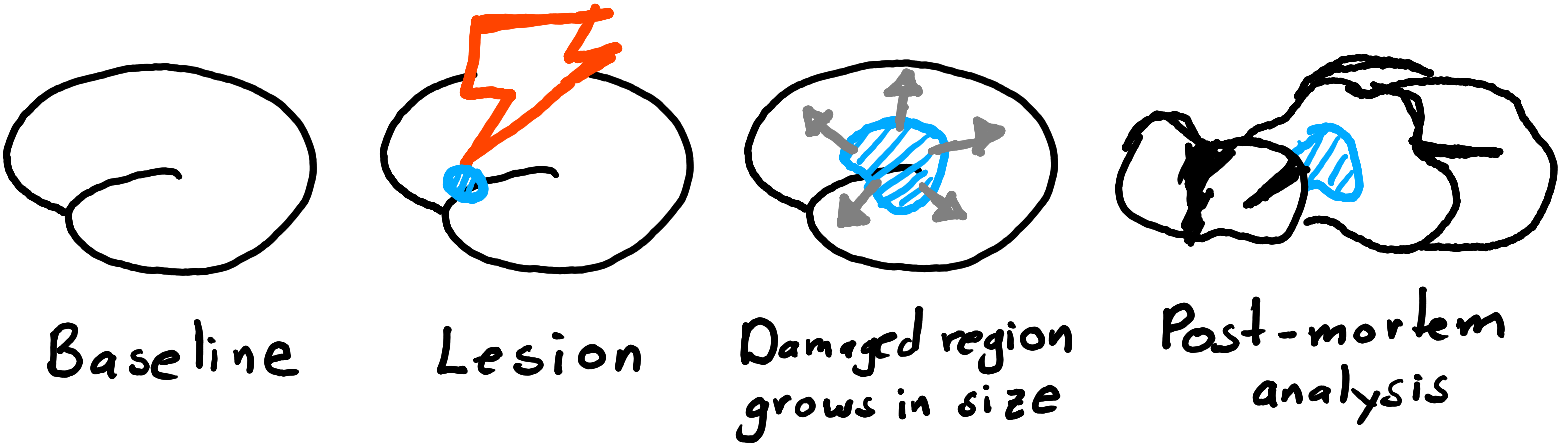
\includegraphics[width=0.8\linewidth]{./img/sketch01_v2}
%\caption{This figure is temporary and will be replaced}
\end{figure}
 

The proposed innovation is to use the information from {symptoms} to enhance the results of ESI.

A posterior analysis of the results of this ESI may be used to aid the identification of the damaged zone as it evolves through time.

This new model considers two phases:
\begin{enumerate}
    \item Static symptoms (finished, reporting now).
    \item Time-changing symptoms.
\end{enumerate}
 



\section{Electrical Source Imaging Formulation}
\begin{itemize}
    \item $N$ dipoles with fixed locations on a grid over the brain volume ($<5$ mm between points).
    \item Each dipole is written as the sum of 3 dipoles with canonical orientations and magnitude to be determined.
    \item $M$ EEG sensors at fixed locations over the head surface.
    \item $T$ time-points, labeled from 1 to $T$.
\end{itemize}
%\begin{figure}
%\centering
%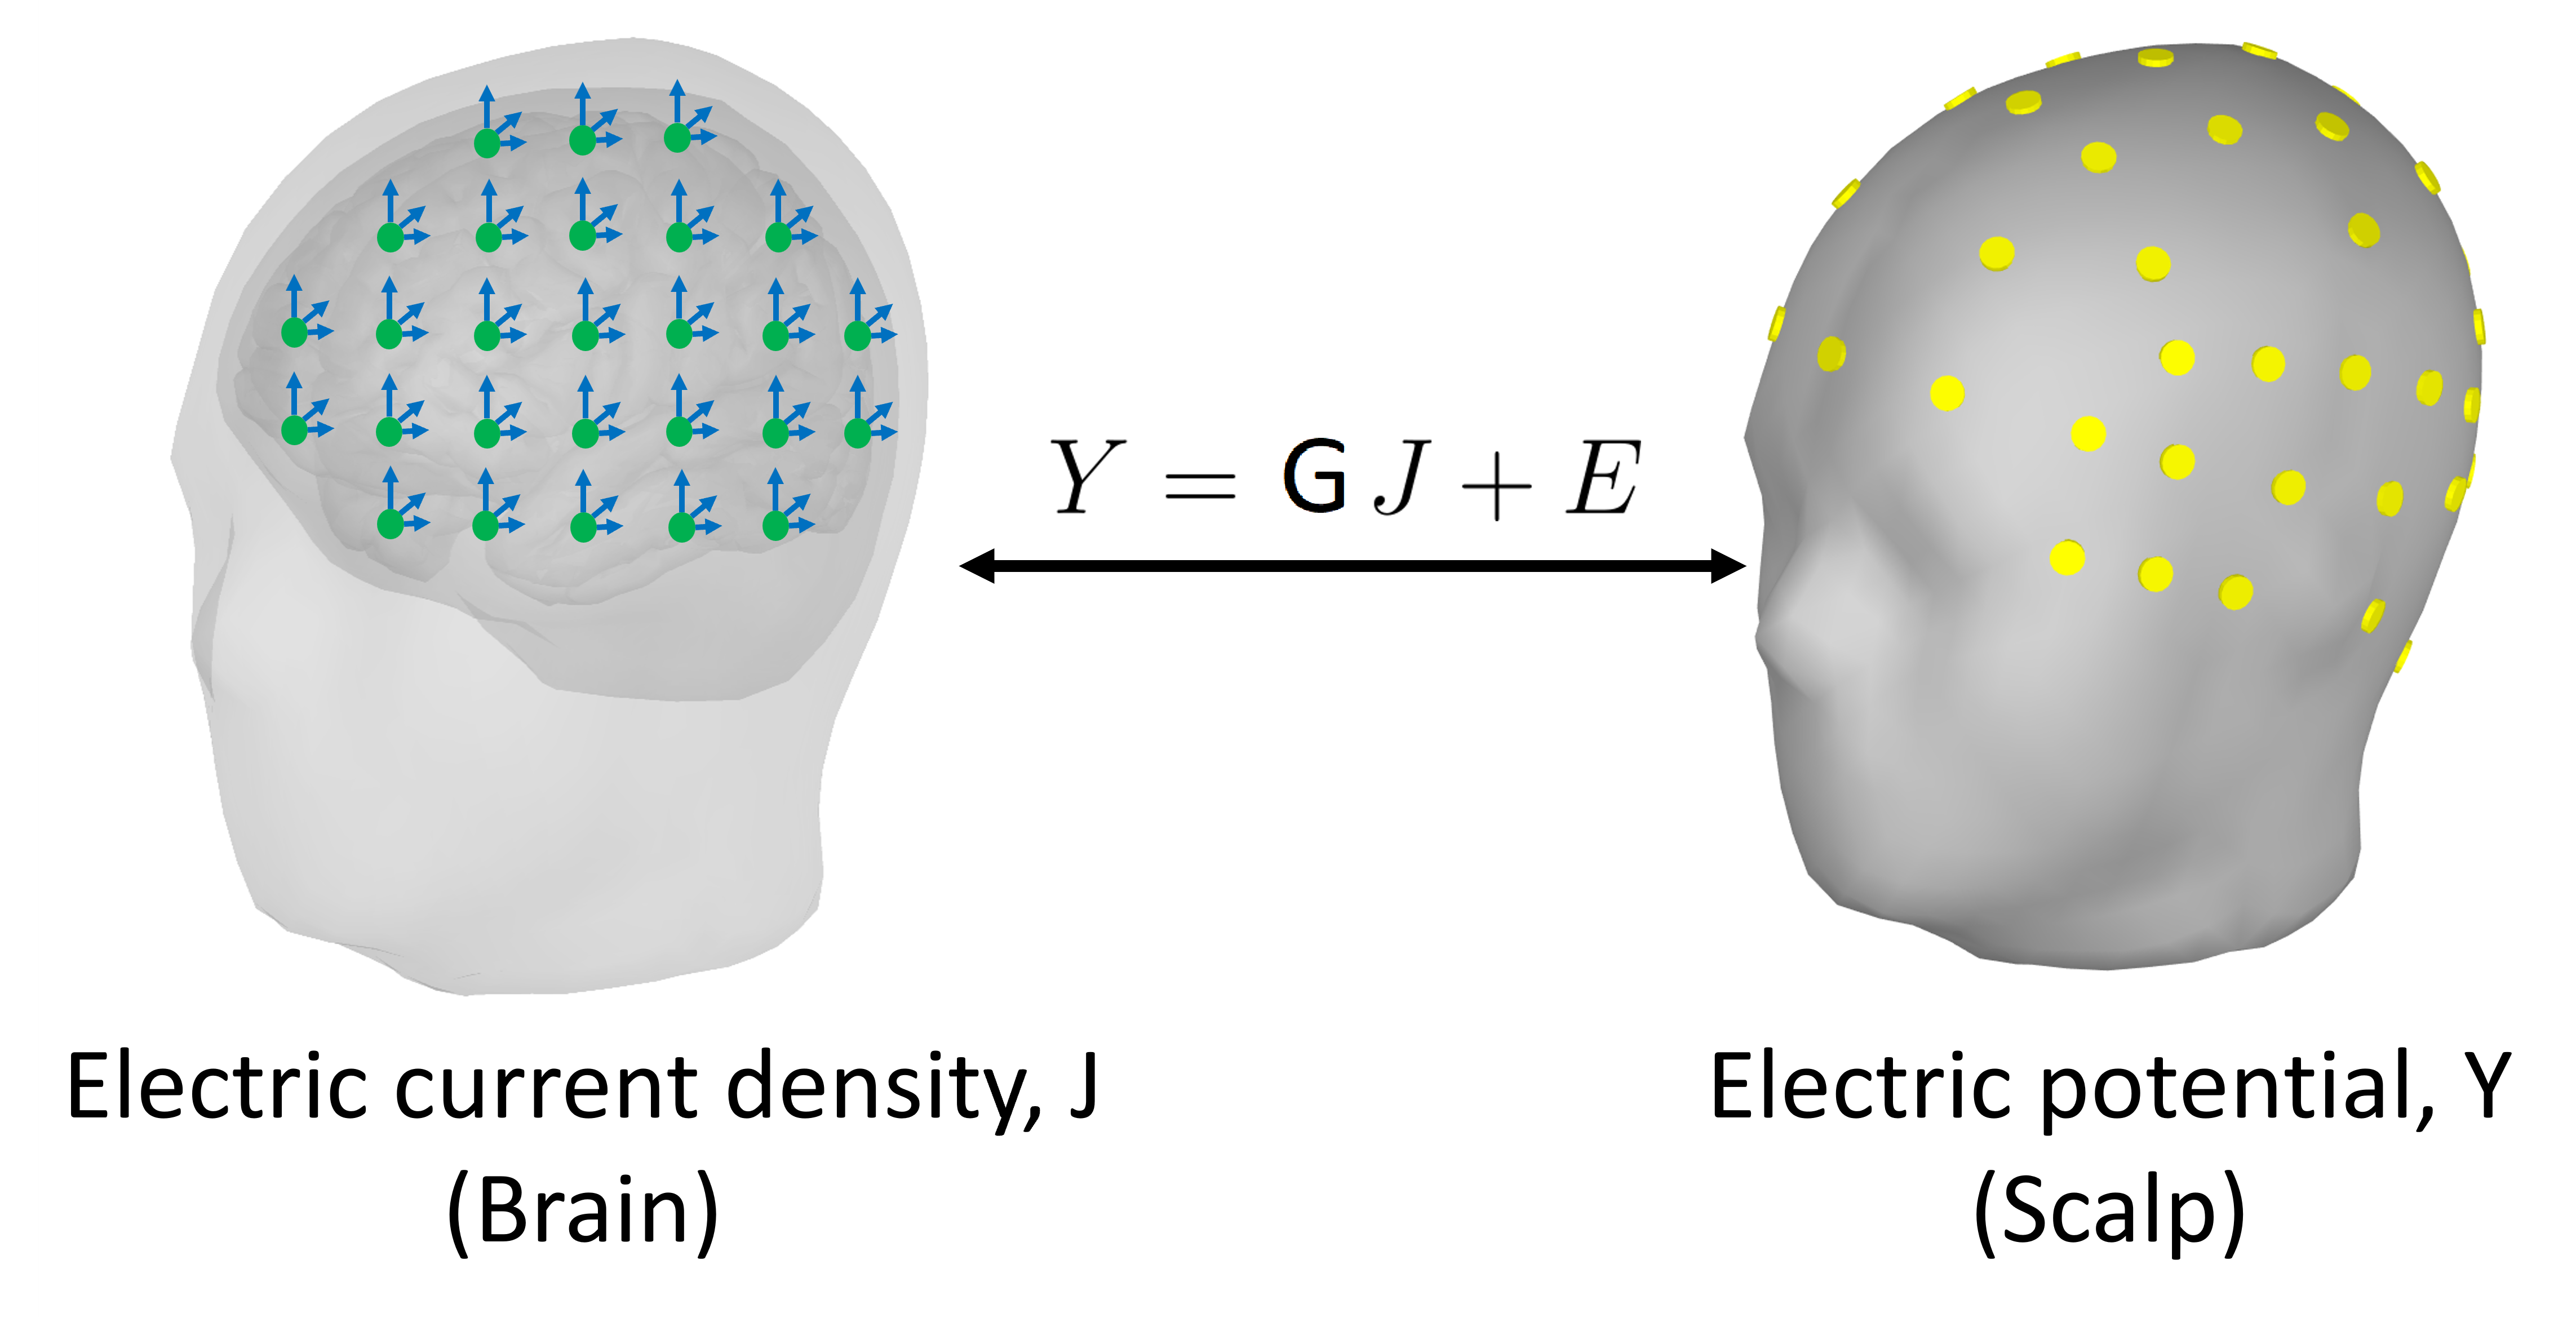
\includegraphics[width=0.5\linewidth]{./img/inverse_prob_v2}
%%\caption{My idea is to make a small variat}
%\end{figure}
 

 {Electrical Source Imaging Formulation}
\textbf{Forward problem}, $N$ unconstrained dipoles with fixed locations
\begin{equation}
\Y = \G \J + \varepsilon.
\end{equation}
where
\begin{itemize}
\item $\Y \in \R^{M \times T}$: EEG measurements.
\item $\J \in \R^{3N \times T}$: Dipole magnitudes, 3 dipoles per grid point.
\item $\G \in \R^{3N\times M}$: `Leadfield matrix', originated from the numerical solution of a Poisson PDE on 3 nested media.
\item $\varepsilon\in \R^{M\times T}$: Additive noise at the sensors.
\end{itemize}
 

% {Notation clarification}
%\begin{itemize}
%\item ${\Y_m(t) \ppar{\in \R}} = e_m^T \Y e_t$: measurement of sensor $m$ at time-point $t$
%\item $\Y(t) \in \ppar{\R^{M\times 1}} = \Y e_t$: vector of all sensor measurements at the time-point $t$
%\item $\Y_m \in \ppar{\R^{1\times T}} = e_m^T \Y$: vector of all measurements of sensor $m$ over time
%\end{itemize}
%
%This notation extends to both $\U$ and $\J$, but it won't be used for other matrices. 
% 

 {Observed symptoms}
The post-mortem observations, which will be referred to as  {symptoms}, are registered against a template brain. 

This information is used to label the dipoles in the grid using
${S\in \set{0,1}^{N\times 1}}$, so that $S_n = 1$ if the $n$-th dipole is located on a region where symptoms were observed.

\begin{figure}
\centering
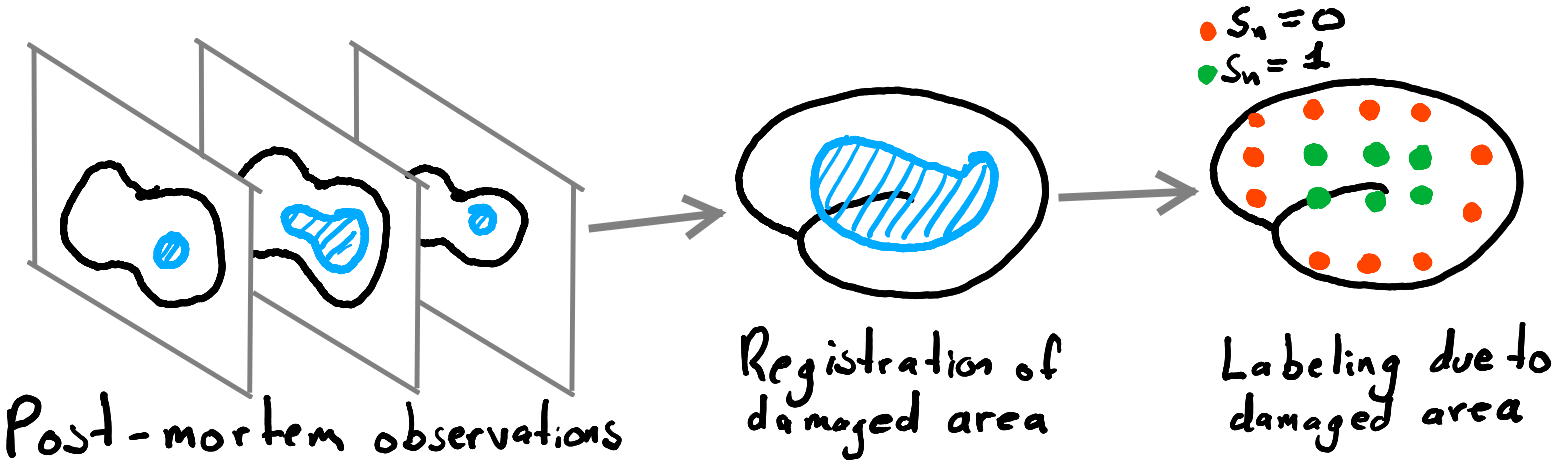
\includegraphics[width=0.8\linewidth]{./img/sketch02_v2}
\end{figure}

 

 {Regional Parcellation}
The  brain is divided into $K$ arbitrary regions. For this work, the Desikan-Killian anatomical atlas is used.
%due to its physiological interpretation. 

Let $R_k$ be all the dipoles in the $k$-th region. Define the matrix $L\in \set{0,1}^{N\times K}$ as
\begin{equation}
    L_{n,k} = \begin{cases}
        1, &\text{if } n\in R_k \\
        0, &\text{otherwise.}
    \end{cases}
\end{equation}

\begin{figure}
\centering
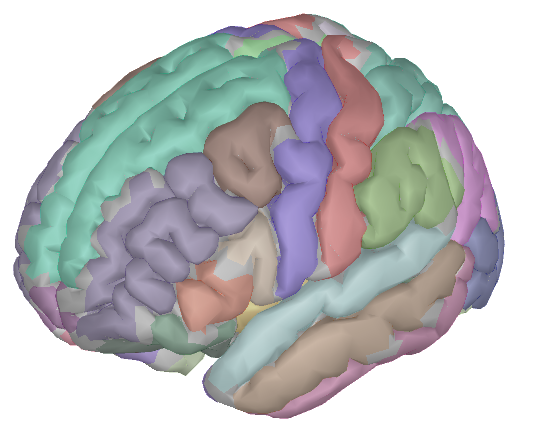
\includegraphics[width=0.3\linewidth]{./img/desikan}

\end{figure}

 

 {Effect of Observed Symptoms}
The relation between symptoms and current density ($\J$) is modeled by adjusting the expected value of the latter based on the symptoms label ($S$).
\begin{equation}
    E\spar{\J_{t,n}} = 
    \begin{cases}
        \U_{t,k} & \text{if } S_n=1 \text{ and } n\in R_k \\
        0 & \text{if } S_n=0
    \end{cases}
\end{equation}
%with $\U \in \R^{K\times T}$ a the collection of regional averages. 
%Thus any dipole located on a region with no symptoms is treated as generating only noise with low amplitude.

This formulation is equivalent to stating that
\begin{equation}
    \J = \text{diag}\ppar{S} L \U + \N
\end{equation}
where $\mathbf{U}\in \R^{K\times T}$ and $\mathbf{N}\in \R^{N\times T}$ are independent and satisfy
\begin{equation}
    \text{Var}\ppar{\N_{t,n}} \ll \text{Var}\ppar{\U_{t,k}}.
\end{equation}
 

 {Distributions from the model}
The proposed model is driven by the following equations
\begin{align}
    \Y &= \G \J + \varepsilon \\
    \J &=  L_S \U + \N
\end{align}
where $\Y, \G$ and $L_S = \text{diag}\ppar{S} L$ are given, and
\begin{align}
    \varepsilon_t &\sim  \norm\ppar{0, \sigma^2 \id } \\
    \N_t &\sim  
    \norm\ppar{0, \gamma_0^2 \id } \\
    \U_t &\sim  
    \norm\ppar{0, \gamma_1^2 \id } 
\end{align}
with $\gamma_0^2 \ll \gamma_1^2$.
 


 {Additional assumption}
For simplicity, assume that
the measurements are generated independently over time, so
%\begin{equation}
%    P\ppar{ \U_t \Big| \U_s } = P\ppar{ \U_t },
%    \text{ if } t\neq s
%\end{equation}
%for any $t, s$. The analogous holds for $\varepsilon$ and $\N$.
\begin{equation}
    P\ppar{ \U } = \prod_{t=1}^T P\ppar{ \U_t }
\end{equation}
The analogous holds for $\varepsilon$ and $\N$.
 

 {Maximum A Posteriori (MAP) estimator}
The estimator is derived from maximizing the a posteriori probability,
\begin{align}
    \ppar{ \hat{\U}, \hat{\N} } &=
    %\set{ \hat{\J}, \hat{\ga} } &=
    \argmax_{\U, \N }\,
    %\argmax_{\J, \ga}\,
    \log P\ppar{\ppar{ {\U}, {\N} } \Big| {\Y; \gamma_0, \gamma_2} }
\end{align}
which derives into the following error function
\begin{align}
    F\ppar{ {\U}, {\N};  \gamma_0, \gamma_1} &=
    \frac{1}{2\sigma^2}
    \nnorm{\G L_S \U + \G \N - \Y}_F^2
    \nonumber \\
    &\phantom{=}
    +
    \frac{1}{2\gamma_0^2} \nnorm{\N}_F^2
    +
    \frac{1}{2\gamma_1^2} \nnorm{L_S \U}_F^2
\end{align}
 


 {Maximum A Posteriori (MAP) estimator}
    The iterative minimization of the error function can be interpreted as a multi-scale iterative correction
    \begin{align}
        \hat{\N}^{(i+1)} &= \argmin_{\N} F\ppar{\U^{(i)},\N; \gamma_0, \gamma_1}
        \\
        \hat{\U}^{(i+1)} &= \argmin_{\U} F\ppar{\U,\N^{(i)}; \gamma_0, \gamma_1}
    \end{align}
    These steps have the following closed form
    \begin{align}
        \hat{\N}^{(i+1)} &=
        \hat{\N}^{(i)}
        -
        \G^T \spar{\G \G^T + \frac{\gamma_0^2}{\sigma^2} \id}^{-1} L_S \ppar{\hat{\U}^{(i)}-\hat{\U}^{(i-1)} }
        \\
        \hat{\U}^{(i+1)} &=
        \hat{\U}^{(i)}
        -
        L_S^T \G^T \spar{\G L_S L_S^T \G^T + \frac{\gamma_1^2}{\sigma^2} \id}^{-1} \ppar{\hat{\N}^{(i)}-\hat{\N}^{(i-1)} }
    \end{align}
 


